ATLAS (a not terribly natural acronym for ``A Toroidal LHC Apparatus'') is a general purpose detector designed to maximize the detection efficiency of all physics objects, including leptons, jets, and photons. This means it is capable of measuring all SM particles, with the exception of neutrinos, the presence of which can be inferred based on missing transverse momentum. The detector measures 44 m long, and 25 m tall. 

The ATLAS detector consists of multiple layers, each of which serves a different purpose in reconstructing collisions. At the very center of the detector is the interaction point where the proton beams of the LHC collide. 

\begin{figure}[H]
\centering
   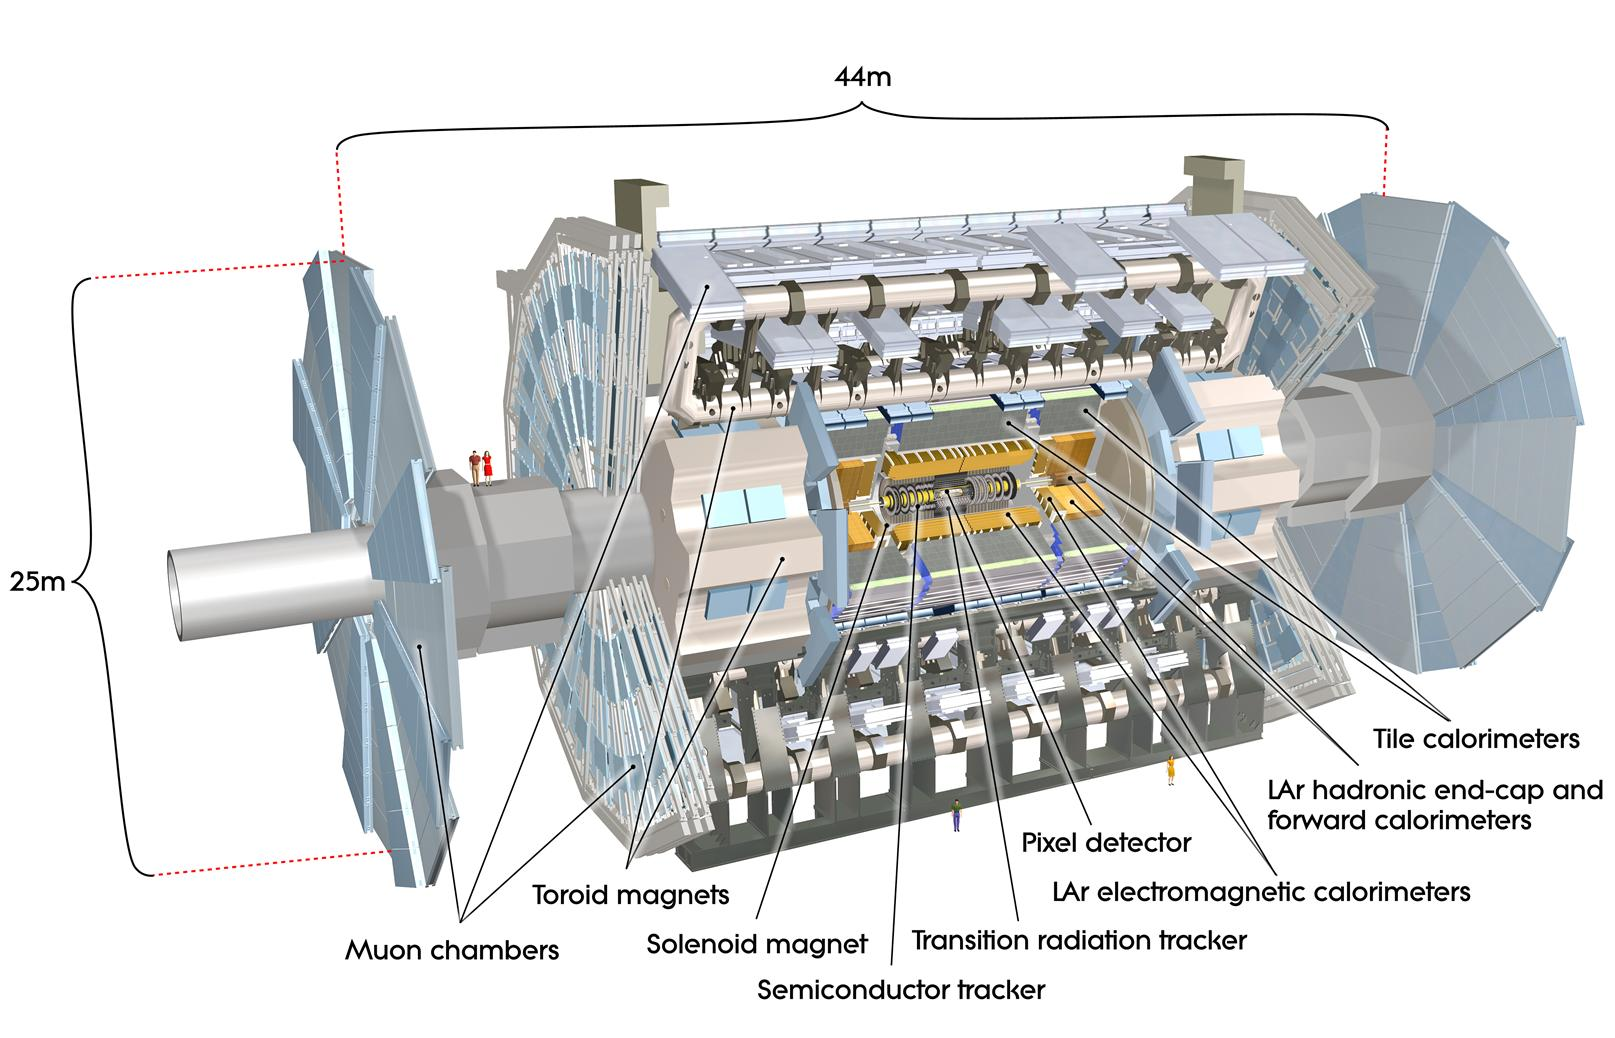
\includegraphics[width=0.75\linewidth]{figures/lhc/ATLASdiagram.eps}
\caption{Cutaway view of the ATLAS detector, with labels of its major components \cite{ATLAS_figure}.}
\label{fig:ATLAS}
\end{figure}

\subsection{Inner Detector}
\label{sec:innerDetector}

\begin{figure}[H]
\centering
   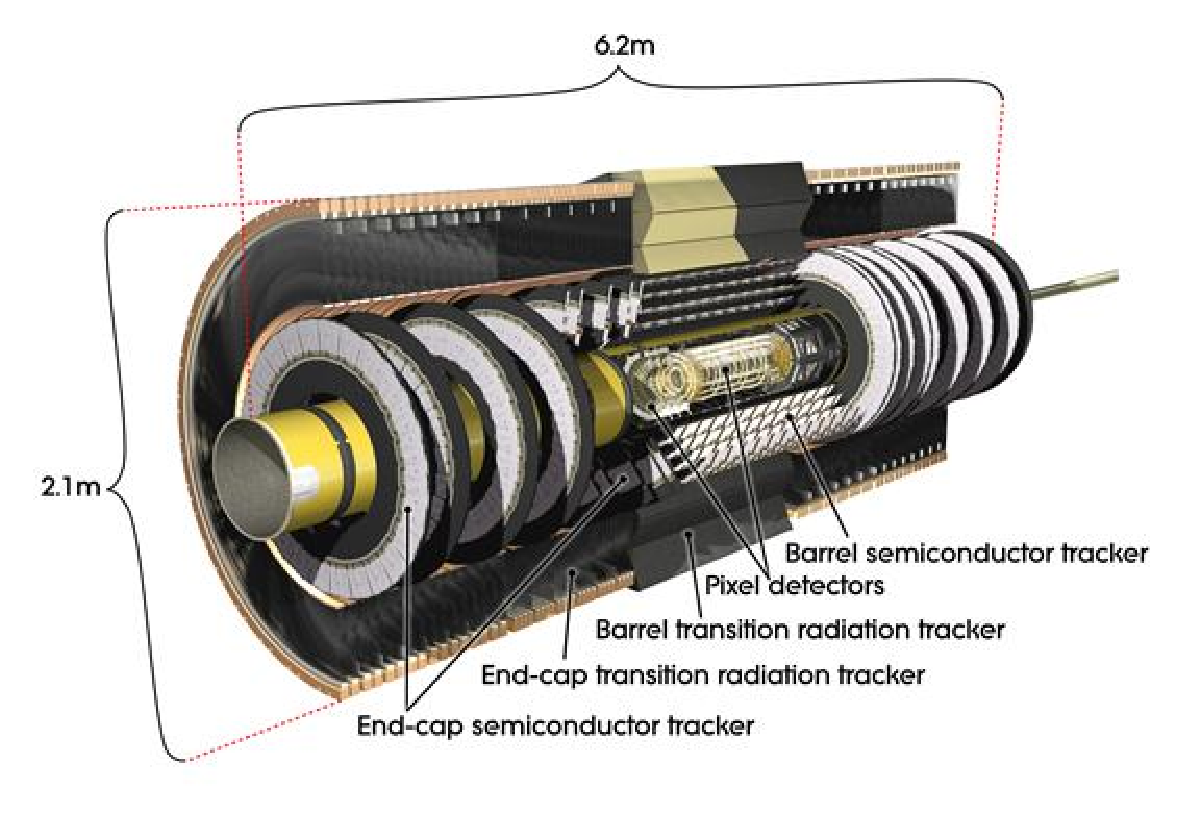
\includegraphics[width=0.75\linewidth]{figures/lhc/InnerDetector.eps}
\caption{Cutaway view of the Inner Detector \cite{caloFig}.}
\label{fig:innerDect}
\end{figure}

Just surrounding the interaction point is the Inner Detector, designed to track the path of charged particles moving through the detector. An inner solenoid surrounding the Innder Detector is used to produces a magnetic field of 2 T. This large magnetic field causes the path of charged particles moving through the Inner Detector to bend. Because this magnetic field is uniform and well known, it can be used in conjunction with the curvature of a particles path to measure its charge and momentum.

The Inner Detector consists of three components - the Pixel Detector, the Semi-Conductor Tracker (SCT), and the Transition Radiation Tracker (TRT). The Pixel Detector is the innermost of these, beginning just 33.25 mm away from the beam line. It consists of three silicon layers along the barrel, as well as three endcap layers, covering a range of $|\eta|$ < 2.5. 

The Semiconductor Tracker (SCT) is similar to the Pixel detector, but uses long strips rather than small pixel to cover a larger spatial area.

\subsection{Calorimeters}
\label{sec:calo}

\begin{figure}[H]
\centering
   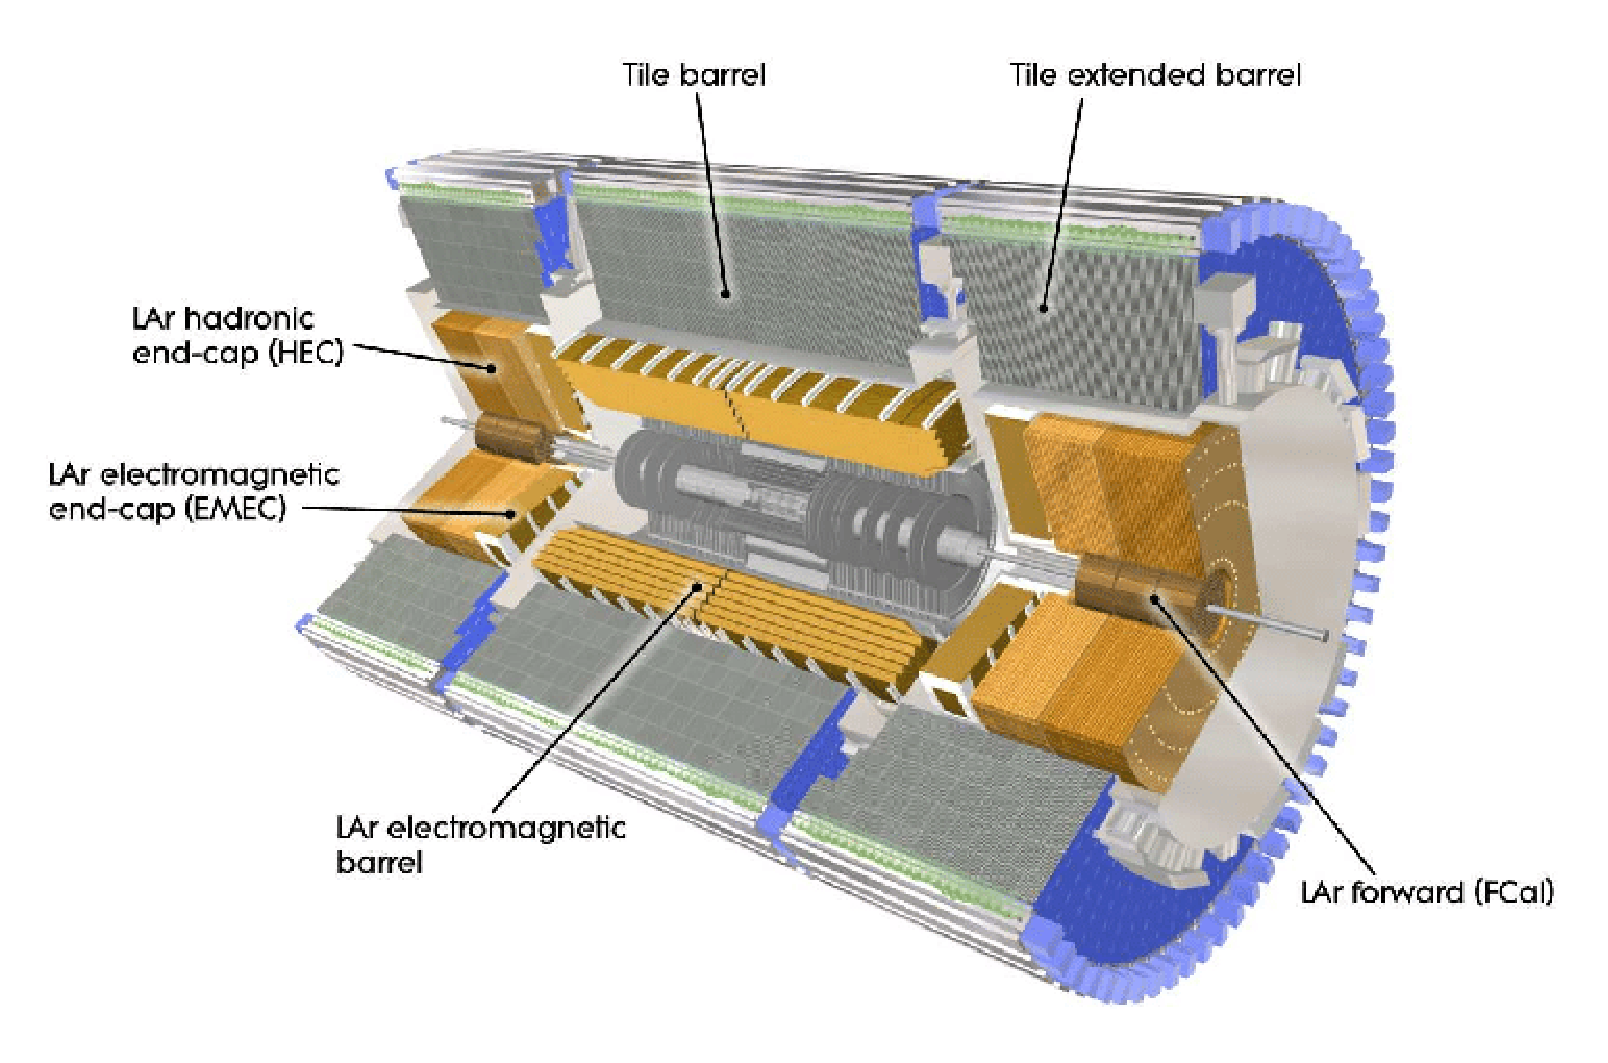
\includegraphics[width=0.9\linewidth]{figures/lhc/calorimeter.eps}
\caption{Cutaway view of the calorimeter system of the ATLAS detector \cite{caloFig}.}
\label{fig:calo}
\end{figure}

Situated outside the Innder Detector are two concentric calorimeters. The inner calorimeter uses liquid argon (LAr) to measure energy of particles the interact electromagnetically, which includes photons and any charged particle. The LAr calorimeter is made of heavy metals, primarily lead and copper, which causes electromagnetically interacting particles to shower, depositing their energy in the detector. The showering of the high energy particles that pass through calorimeter cause the liquid argon to ionize, and the ionized electrons are detected by electronic readouts. The LAr calorimeter consists of around 180,000 readout channels.  

The outer calorimeter measures the energy from particles that pass through the EM calorimeter, and measures the energy of particles that interact via the strong force. This is primarily hadrons. It is composed of steel plates to cause hadronic showering and scintillating tiles as the active material. The signals from the hadronic calorimeter are read out by photomultiplier tubes (PMTs).

\subsection{Muon Spectrometer}
\label{sec:muonSpec}

Because muons are heavier than electrons and photons, and do not interact via the strong force, they generally pass through the detector without being stopped by the calorimeters. The outermost components of the detector are designed specifically to measure the energy and momentum of muons produced in the LHC. The muon spectrometer consists of tracking and triggering system. It extends from the outside of the calormeter system, about a 4.25 m radius from the beam line, to a radius of 11 m. This large detector system is necessary to accurately measure the momentum of muons, which is essential not only for measurements involving the muons themselves, but also to accurately estimate the missing energy in each event.

Two large toroidal magnets within the muon system generate a large magnetic field which covers an area 26 m long with a radius of 10 m. Because the area covered by this magnet system is so large, a uniform magnetic field like the one produced in the Inner Detector is impractical. Instead, the magnetic field that exists in the muon spectrometer ranges between 2 T and 8 T, and is much less uniform. The path of the muons passing through the spectrometer is bent by this field, allowing their charge to be determined. 

1200 tracking chambers are placed in the muon system in order to precisely measure the tracks of muons with high spatial resolution.

%\subsection{Forward Detector}
%\label{sec:forwardDet}

\subsection{Trigger System}
\label{sec:trigger}

Because of the high collision rate and large amount of data collected by the various subdetectors, ATLAS produces far more data than can actually be stored. Each event produces around 25 Mb of raw data, which multiplied by the bunch crossing rate of 40 MHz, comes out to around a petabyte of data every second. The information from every event cannot practically be stored, therefore a sophisticated trigger system is employed in real time to determine whether events are sufficiently interesting to be worth storing.

The trigger system in ATLAS involves multiple levels, each of which select out which events move on to the next level of scrutiny. The level-1 trigger uses hardware information from the calorimeters and muon spectrometer to select events that contain candidates for particles commonly used in analysis, such as energetic leptons and jets. The level-1 trigger reduces the rate of events from 40 MHz to around 100 kHz. 

Events that pass the level-1 trigger move to the High-Level Trigger (HLT). The HLT takes place outside of the detector in software, and looks for properties such as a large amount of missing transverse energy, well defined leptons, and multiple high energy jets. Events that pass the HLT are stored and used for analysis. Because the specifics of the HLT are determined by software rather than hardware, the thresholds can be changed throughout the run of the detector in response to run conditions such as changes to pilup and luminosity. After the HLT is applied, the event rate is reduced to around 1000 per second, which are recorded for analysis.
